\section{Fazit}

In dieser Arbeit haben wir versucht, mithilfe von Grafana, Loki und Promtail eine \gls{SIEM}-Lösung zu emulieren, um Überwachungsmechanismen anhand von Logdateien zu erstellen. In der folgenden Tabelle zeigen wir die Rolle jedes verwendeten Tools bei der Erreichung unseres Ziels:

\begin{table}[h]
    \centering
    \setstretch{1.2}
    \begin{tabular}{|c|c|}
    \hline
    \textbf{Tool}    & \textbf{Funktionalität}         \\ \hline
    Promtail         & Datensammlung                   \\ \hline
    Loki             & Normalisierung und Vearbeitung  \\ \hline
    Grafana          & Berichts- und Grafikgenerierung \\ \hline
    Grafana:Alerting & Generierung von Warnmeldungen   \\ \hline
    \end{tabular}
    \caption{Verwendete Tools und ihre Hauptfunktionalitäten} 
    {Verwendete Tools und ihre Hauptfunktionalitäten}
    \label{tab:VerewendeteTools}
\end{table}

Wir stellen fest, dass die verwendeten Tools trotz einiger Einschränkungen eine kosteneffektive Möglichkeit bieten, ein Überwachungssystem zu implementieren. Die Methoden zur Erkennung von Angriffen lassen sich anhand der \glsfirst{ttp} der \gls{mitre} Matrix definieren. Nach der Auswahl eines Angriffs erstellen wir Regelwerke mit der Abfragesprache \gls{logql} in Loki, um Muster zu identifizieren, die auf den ausgewählten Angriff hindeuten. Diese Regelwerke werden dann verwendet, um Warnmeldungen über den Angriff zu generieren und zu versenden.

Die Einschränkungen beziehen sich auf verschiedene Probleme in der neueren Version von Loki, die seit 2022 gemeldet wurden und für die bisher keine Lösung existiert.

\subsection{Herausforderungen}
Die korrekte Erstellung der Regelwerke stellt die größte Herausforderung bei dieser Implementierung dar. Um die Tools präzise anzuwenden, ist es entscheidend, die Regelwerke richtig zu entwickeln, um potenzielle Angriffe identifizieren zu können. Da Logdateien aus produktiven Umgebungen eine große Menge an Informationen enthalten, müssen die Regelwerke so definiert werden, dass sie die relevanten Informationen wie IP-Adresse, Portnummer, Zeitfenster und Zeitabstände zwischen Anfragen filtern und nach Angriffsmustern kategorisieren können. Die Lernkurve für den Aufbau der richtigen Regelwerke kann eine große Herausforderung darstellen, wie auch in unserem Fall.

Die korrekte und präzise Indexierung spielt eine entscheidende Rolle für die Leistung der Anwendung. Die Verwendung vieler Labels erfordert eine hohe Rechenkapazität und kann auch zu fehlerhaften Ergebnissen führen, wie bei uns. Die Rechenkapazität muss ebenfalls angepasst werden, um sicherzustellen, dass die steigende Anzahl von Anfragen (siehe Abbildung \ref{fig:Eskalation_Labels} auf Seite \pageref{fig:Eskalation_Labels}) nicht zu Abstürzen führt.

\subsection{Zukünftige Forschung}

Die von uns definierten Regeln basieren auf statischen Elementen wie der \quotes{Anzahl von Anfragen}, dem \quotes{Zeitabstand zwischen Requests} und der \quotes{Anzahl von fehlgeschlagenen Anmeldeversuchen}. Moderne Angriffe haben jedoch auch einen dynamischen Aspekt, der sich an die Umgebung anpasst, insbesondere durch die fortschreitende Entwicklung von \glsfirst{KI} \citep{Guembe_AIHACKER}.

\gls{KI} kann zur Automatisierung von Aufgaben oder zur effizienten Datenanalyse eingesetzt werden. Für die zukünftige Weiterentwicklung dieser Arbeit kann dieses Werkzeug eine große Unterstützung bieten, indem es performantere und effizientere Regelwerke vorschlägt, um die Log-Analyse effizienter und zuverlässiger zu gestalten. Dies würde dazu beitragen, einen sicheren Netzwerkverkehr zu gewährleisten.


%Während \gls{KI} einerseits für die Automatisierung von Aufgaben oder für effiziente Datenanalyse verwendet wird, könnte sie auch für Cyberkriminalität genutzt werden. \gls{KI} ist am Ende nur ein Werkzeug, dessen Nutzung von den Absichten ihrer Benutzer abhängt.




% % % Verschiedene Angriffstechniken lassen sich schneller und effizienter mit \gls{KI} durchführen. Die Nutzung von \gls{polyphomicMalware} ist ein Beispiel, wo weder Antivirus-Programme noch Log-Analyse-Tools einen normalen von einem abnormalen Ablauf unterscheiden können. Auch die Verkehrsanalyse kann durch \gls{KI} gefährdet sein, da Angriffe und normaler Verkehr ähnlich dargestellt werden können. Darüber hinaus kann \gls{KI} auch gegen Authentifizierungsverfahren eingesetzt werden, um beispielsweise Anmeldedaten schneller zu \gls{bruteforce} und/oder vorauszusehen \citep{Fritsch_AIcybersec}.

% \newpage
% Das folgende Diagramm zeigt, wo sich \gls{KI} bei Cyberangriffen anhand der\gls{CKC} integrieren lässt:


% \begin{figure}[H]
%     \centering
%     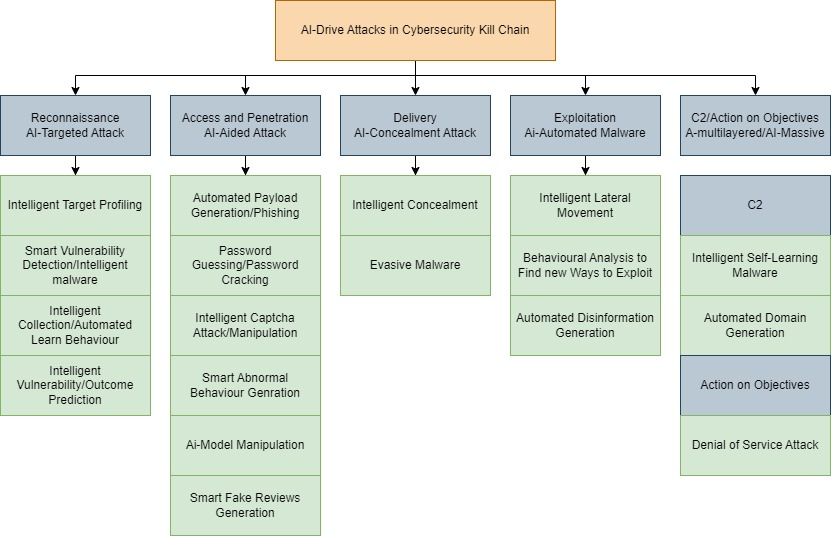
\includegraphics[width=0.9\textwidth]{assets//CKC_AI.jpg}
%     \caption[\gls{KI} in der \glsfirst{CKC}]
%     {\gls{KI} in der \glsfirst{CKC}\\Quelle: \citep{Guembe_AIDiagrammAngriff}}
%     \centering
%  \end{figure}
 

% Um sicherzustellen, dass unsere Lösungen sich an diese neue und dynamische Realität anpassen können, können zukünftige Regelsätze mithilfe von \gls{KI} erstellt werden. Nachdem die meisten möglichen Angriffsflächen identifiziert wurden, sollten die Regeln die viele mögliche Szenarien abdecken.

% Mit der rasanten Entwicklung von \gls{KI}, insbesondere während der Erstellung dieser Arbeit, können wir auch erwarten, dass sich sowohl Loki als auch Grafana bald mit verschiedenen \gls{opensource} \gls{plugin} integrieren lassen, die auch \gls{KI} unterstützen. Diese sollen dazu beitragen, die Loganalyse effizienter und zuverlässiger zu machen. All dies würde dabei helfen, einen sicheren Netzwerkverkehr zu gewährleisten.


